\chapter{Diseño}\label{chap:diseno}

\section{Proyecto como servicio}
Un proyecto como servicio es una aplicación modular y distribuida en la que el backend funciona como un servicio independiente de la plataforma, permitiendo la interacción con varios tipos de clientes (web, móvil, etc.) con conexión a Internet. 

Presenta gran flexibilidad ante la implementación de mejoras, ya que se pueden realizar cambios en el backend sin afectar al frontend, y viceversa. Como puede ser agregar más tipos de análisis de gastos sin afectar al resto del sistema. A medida que los usuarios crecen, el backend puede escalarse fácilmente. Sin embargo, también presenta desventajas, como dependencia de la red, ya que requiere conexión entre cliente y servidor, lo cual puede ser una limitación si el servicio se utiliza sin darse esa condición\cite{galster2014variability}.

Este proyecto sigue un enfoque como servicio, ya que se espera que la aplicación pueda ser utilizada por un número creciente de usuarios y que se puedan implementar mejoras frecuentes y nuevas funcionalidades en el futuro, motivado principalmente desarrollo ágil en el mismo. Además es importante que se disponga de acceso multiplataforma (como se refleja en la Figura \label{fig:proyecto_como_servicio}), puesto que se desarrollarán funcionalidades útiles para dispositivos móviles (como el uso del GPS) y otras más orientadas a su uso en ordenador (como las consultas detalladas de los movimientos realizados por el usuario, donde se obtendrá mayor comodidad para analizar el potencial volumen de datos). En mayo de 2024, un estudio de la CNMC\footnote{Comisión Nacional de los Mercados y la Competencia} reveló que el 80\% de las personas en España acceden diariamente a Internet, por ello se considera que la mayoría de los usuarios de la aplicación tendrán acceso a la red y podrán utilizarla sin problemas\cite{cnmc2024}. 
De este modo, se determina la creación de una \textbf{aplicación web}.

\begin{figure}[ht!]
    \centering
    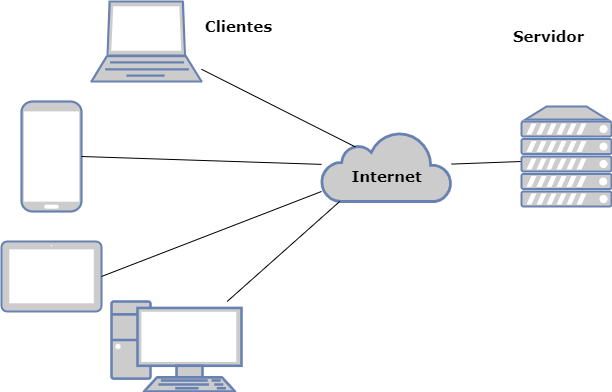
\includegraphics[width=\linewidth]{imagenes/proyecto_servicio.drawio.png}
    \caption{Proyecto como servicio (elaboración propia).}
    \label{fig:proyecto_como_servicio}
\end{figure}


\section{Arquitectura software}\label{sec:arquitectura_software}
La arquitectura software de un proyecto podría definirse como la estructura y organización de los elementos que lo componen, así como las relaciones y dependencias entre ellos. Es un aspecto importante en el diseño de una aplicación, ya que permite orientarla hacia el logro de los objetivos planteados y tiene en consideración la posible evolución del sistema: su comprensión, escalabilidad, mantenimiento y rendimiento\cite{fernandez2006arquitectura}.
Para definir la arquitectura de software de la aplicación, se analizaron varias opciones disponibles, cada una con características y beneficios diferentes\cite{albin2003art}\cite{garimilla2024art}:

\begin{itemize}
\item \textbf{Arquitectura monolítica}\\
Las arquitecturas monolíticas agrupan todos los componentes de la aplicación en una única unidad de despliegue, lo cual facilita la implementación y es adecuado para aplicaciones pequeñas o medianas. Sin embargo, este enfoque suele presentar limitaciones en cuanto a flexibilidad y escalabilidad, ya que todos los módulos están estrechamente acoplados. Lo que provoca que las opciones de actualización y expansión se vean reducidas.

\item \textbf{Arquitectura basada en microservicios}\\
Una arquitectura de microservicios organiza la aplicación en servicios pequeños e independientes que pueden desarrollarse, desplegarse y escalarse de manera autónoma. Cada microservicio puede implementarse con el lenguaje y las herramientas más adecuadas para su función, lo que aporta flexibilidad y facilita la escalabilidad. Además, su naturaleza distribuida añade seguridad, ya que los servicios se pueden comunicar a través de una API y no de manera directa, ofreciendo una capa adicional de protección. Sin embargo, esta estructura aumenta la complejidad de implementación y requiere mayor infraestructura, lo cual puede ser innecesario para aplicaciones como esta con un alcance más específico\cite{RedHat2023}\cite{lopez2017arquitectura}.

\item \textbf{Arquitectura Cliente-Servidor}\\
La arquitectura cliente-servidor divide la aplicación en dos componentes principales: el cliente (interfaz de usuario) y el servidor (lógica de negocio y acceso a datos). La comunicación entre cliente y servidor se puede gestionar mediante una API REST (Representational State Transfer), que utiliza solicitudes HTTP\footnote{HyperText Transfer Protocol: es un protocolo cliente-servidor para comunicar aplicaciones por medio de peticiones de datos y recursos.} (como GET, POST, PUT y DELETE) para intercambiar información. Este enfoque proporciona una separación clara entre la interfaz y la lógica de negocio, facilitando el mantenimiento y la escalabilidad sin necesidad de una infraestructura compleja como en el caso de los microservicios.

\end{itemize}

En una arquitectura de microservicios, cada servicio es independiente, lo cual permite a los equipos de desarrollo elegir el lenguaje de programación y el entorno de ejecución más adecuado para cada servicio, lo que facilita la escalabilidad y la modularidad del sistema. En la de cliente-servidor, sin llegar a ser tan flexible como los microservicios, permite una mayor flexibilidad que la arquitectura monolítica. Por lo que se descarta la implementación de una arquitectura monolítica.

La arquitectura basada en microservicios no se justifica para las necesidades actuales del proyecto, que al resolver una necesidad específica no se beneficia especialmente de las ventajas que ofrece, sin embargo, su desarrollo sí podría verse afectado por la complejidad que añade. 

En su lugar, se ha optado por implementar una arquitectura \textbf{cliente-servidor} para la aplicación. La comunicación entre ambos se realiza mediante una API REST. Esto permite modularidad, escalabilidad, y facilidad de mantenimiento, posibilitando una futura migración a microservicios si es necesario. La API REST en esta arquitectura conecta de forma sencilla y eficiente los datos y funcionalidades del backend con el frontend.


\section{Diseño interfaz de usuario y navegación en la plataforma}
\label{sec:diseno_interfaz_usuario}
La interfaz de usuario es un aspecto fundamental en el diseño de una aplicación, ya que es la primera impresión que recibe el usuario y determina en gran medida su experiencia de uso. Una interfaz bien diseñada debe facilitar la interacción del usuario con la plataforma. Para lograrlo, es necesario definir una estructura clara y coherente, y diseñar una interfaz visual atractiva y funcional.

El siguiente \textit{wireframe} (Figura \ref{fig:wireframes_vistas}) representa las distintas vistas y funcionalidades de la aplicación final, permite visualizar la estructura y el flujo de la misma. Para realizarlo se ha utilizado la herramienta \textit{Moqups}\footnote{\url{https://app.moqups.com/}}, que permite crear wireframes online de forma sencilla. Este boceto es una representación inicial de la interfaz de usuario y puede sufrir modificaciones a lo largo del desarrollo de la aplicación.

\begin{figure}[ht!]
    \centering
    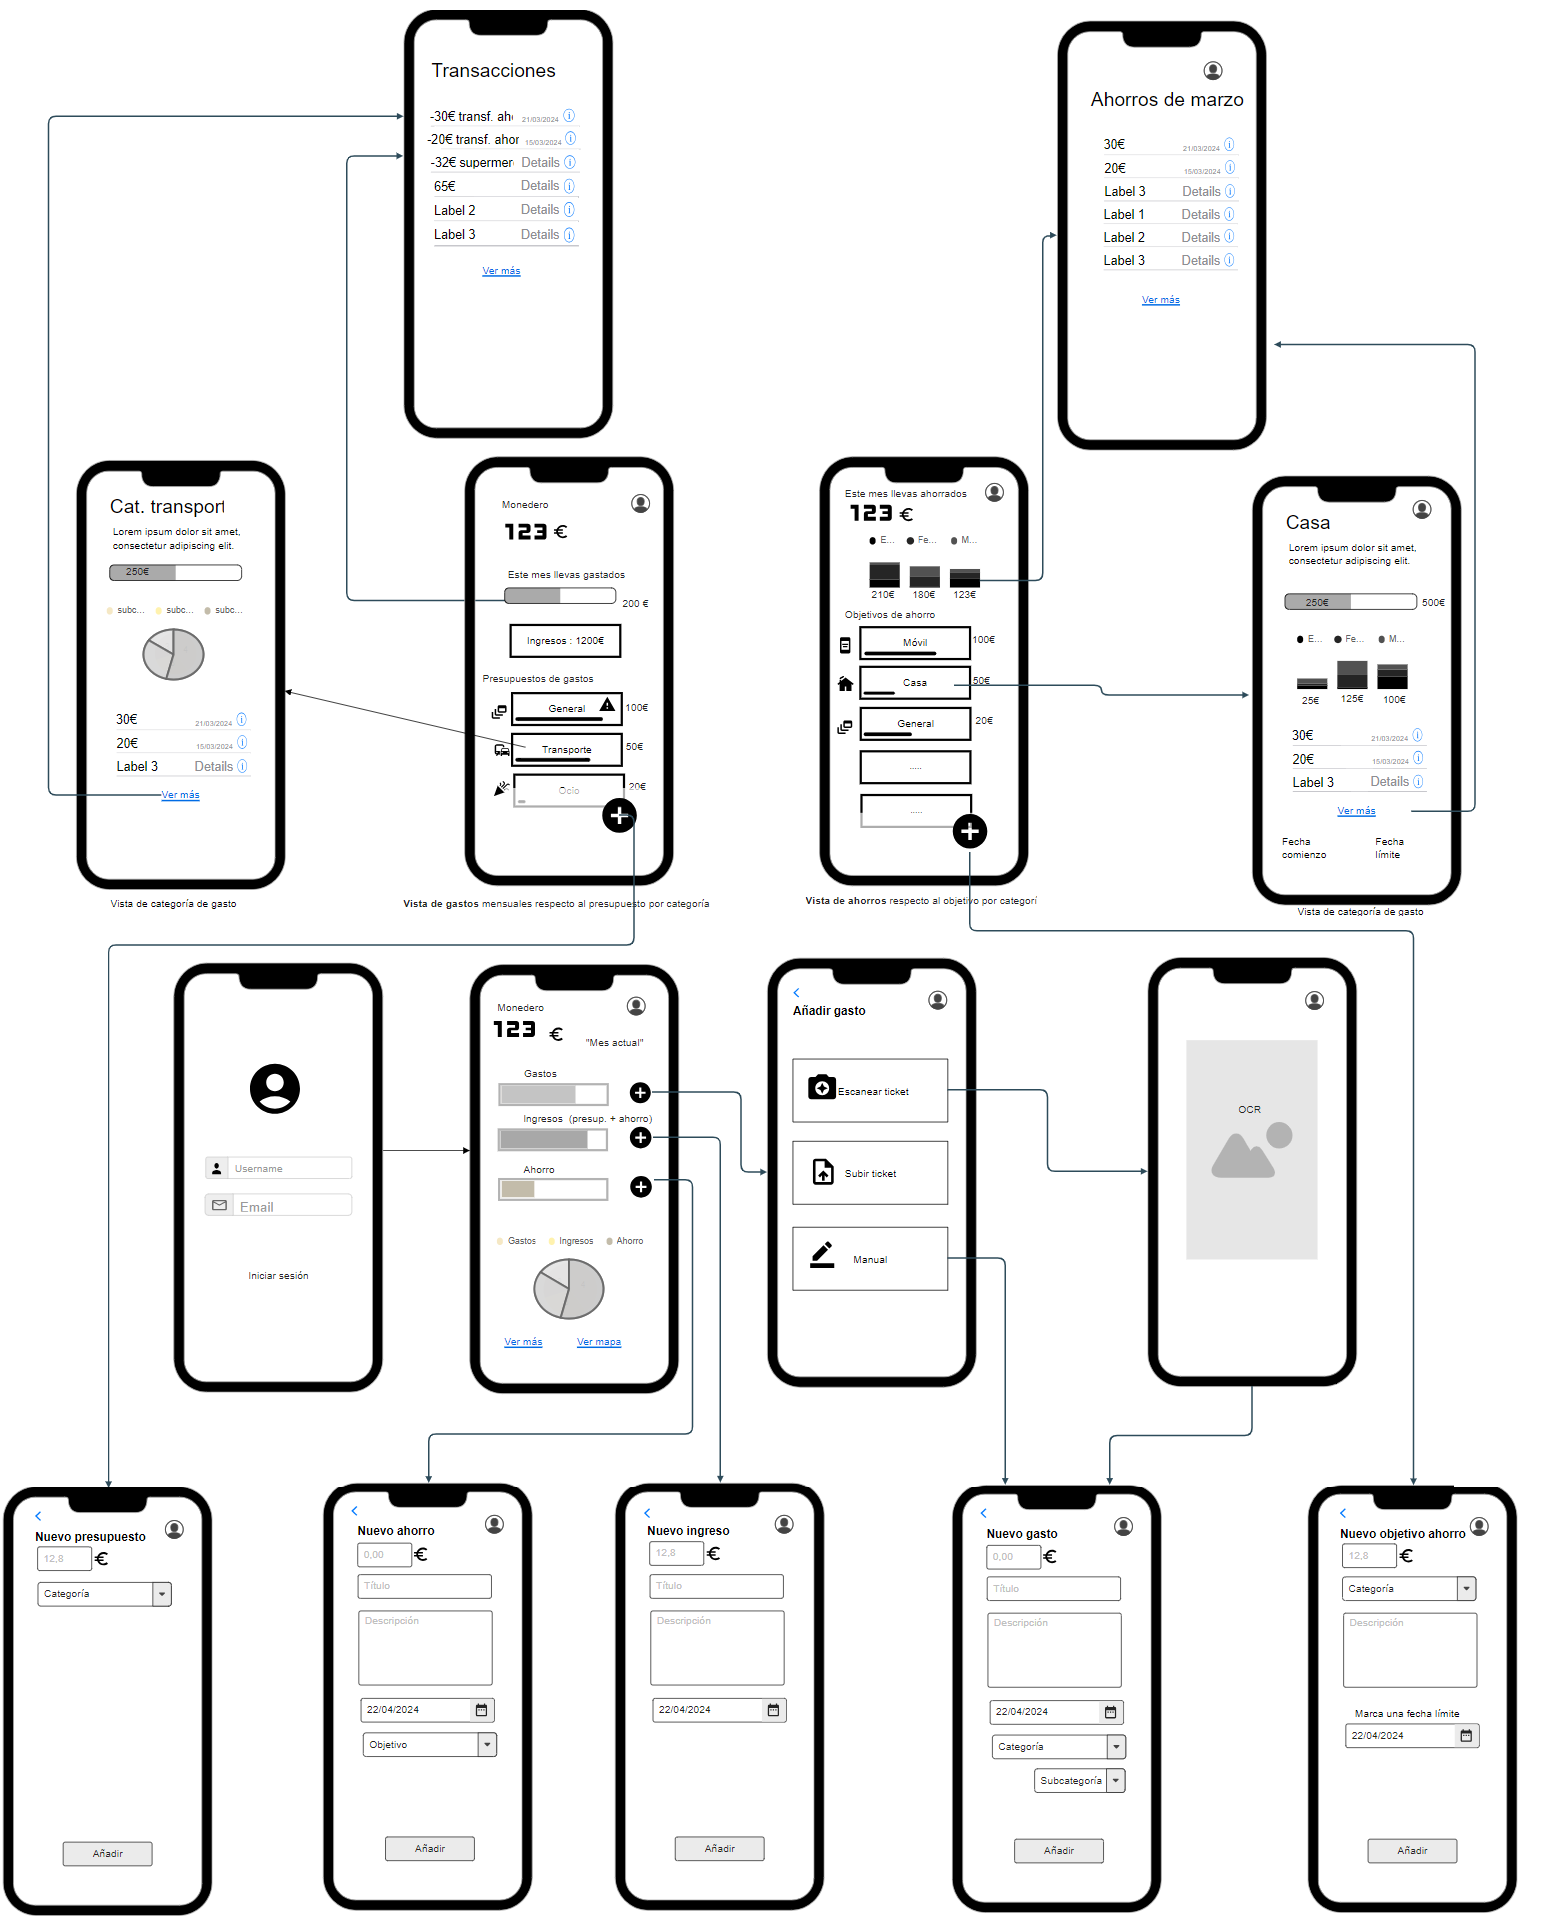
\includegraphics[width=\linewidth]{imagenes/wireframe.moqups.png}
    \caption{Wireframes de la interfaz de usuario en la aplicación (elaboración propia).}
    \label{fig:wireframes_vistas}
\end{figure}



\section{Decisiones estratégicas. Milestone 1}
Una vez definida la arquitectura de la aplicación, las estructuras de datos que se requieren y diseñados los bocetos de la interfaz de usuario, se describen las decisiones estratégicas que determinan la elección de las tecnologías que se usarán en la implementación.


En la arquitectura cliente-servidor adoptada para este proyecto (en la sección \ref{sec:arquitectura_software}), el protocolo \textbf{HTTP} es el estándar que permite la comunicación entre el navegador (cliente) y el servidor web, facilitando que el cliente realice acciones necesarias. 

Para estructurar y regular estas interacciones, se utiliza una API (Application Programming Interface), que define las reglas y protocolos para la comunicación entre aplicaciones a través de la red. En este caso, se emplea una \textbf{API REST} (Representational State Transfer), que sigue los principios de HTTP, organizando las operaciones en torno a recursos específicos y permitiendo la comunicación mediante solicitudes GET, POST, PUT y DELETE. 

Además, la API REST se complementa con un \textbf{ORM} (Object-Relational Mapping), que facilita el manejo de datos entre la aplicación y la base de datos. Permite manipular los datos mediante objetos de la aplicación en lugar de consultas SQL directas, simplificando el trabajo con entidades (como usuarios o transacciones) y reduciendo riesgos de seguridad como inyecciones SQL, también mejora la legibilidad del código.

Por su parte, la \textbf{base de datos} actúa como repositorio central de información para la API REST, almacenando y gestionando todos los datos de la aplicación. La API accede a esta información a través del ORM para responder las solicitudes del cliente. Esta arquitectura modular optimiza el flujo de comunicación entre el usuario y la base de datos\cite{marquez2022backend}.

Para implementar este backend, se requiere seleccionar herramientas que se ajusten a las necesidades específicas del proyecto.

\subsection{Lenguaje de programación}
\subsubsection{Criterios de búsqueda}
Debe tener soporte para el desarrollo de APIs y para la conexión a la base de datos. Además debe ser compatible con bibliotecas de testing y OCR.

\subsubsection{Criterios de selección}
Para las opciones compatibles con los criterios de búsqueda se escogerá preferentemente aquella donde se cumplan la mayor parte o todos los criterios de selección descritos a continuación.

\begin{itemize}
    \item Relación de experiencia / interés en el lenguaje por parte del desarrollador.
    \item Simplicidad en la instalación y uso de OCR.
\end{itemize}

\subsubsection{Opciones compatibles con los criterios de búsqueda}
\begin{itemize}
    \item \textbf{Python}\\
        Aunque el desarrollador no tiene a penas experiencia con el lenguaje, es conocido por su simplicidad y legibilidad, lo que facilita el desarrollo y mantenimiento del código. Respecto al OCR, Python tiene una ventaja significativa gracias a Pytesseract, una interfaz para Tesseract fácil de usar, con buenos resultados y ampliamente usada para el procesamiento de imágenes.
    \item \textbf{JavaScript} (Node.js)\\
        En comparación con Python, JavaScript puede tener una curva de aprendizaje más pronunciada. Además, el desarrollador tiene menos experiencia desarrollando aplicaciones web en JavaScript que en Python.
    \item \textbf{Java}\\
        La configuración y el desarrollo de una aplicación web en Java pueden requerir más tiempo y esfuerzo en comparación a los anteriores. Aunque el conocimiento del desarrollador en Java es mayor que en Python o JavaScript.
\end{itemize}

\subsubsection{Opción seleccionada y justificación}
Para el desarrollo de la aplicación se ha seleccionado \textbf{Python} como lenguaje de programación. Python cumple con todos los criterios de búsqueda y selección. Además, ofrece una amplia gama de bibliotecas y herramientas para el desarrollo de APIs\cite{python2021python}. A pesar de no ser el lenguaje de programación más conocido por el programador, su uso extendido en la actualidad motiva al desarrollador a indagar más él, poniendo esta opción por encima del resto. 


\subsection{Framework de backend}
\subsubsection{Criterios de búsqueda}
Debe estar optimizado para crear APIs de forma rápida y eficiente.
Debe ofrecer compatibilidad con el lenguaje de programación elegido (Python). También debe contar con integración de ORMs.

\subsubsection{Criterios de selección}
\begin{itemize}
    \item Se valorará positivamente la facilidad para documentar y si dispone de un entorno para pruebas.
    \item Se prioriza un framework que gestione eficientemente las solicitudes HTTP, con soporte para programación asíncrona, de forma que se optimice el rendimiento a la hora de atender gran número de solicitudes de forma simultánea.
\end{itemize}

\subsubsection{Opciones compatibles con los criterios de búsqueda}
\begin{itemize}
    \item \textbf{FastAPI}\\
        Fue diseñado específicamente para la creación de APIs de alto rendimiento y maneja solicitudes HTTP de manera eficiente al soportar asincronía nativa.
        Genera documentación de forma automática, lo que simplifica la validación y pruebas de los endpoints.
    \item \textbf{Django}\\
        Permite crear documentación, pero no se genera de forma automática, lo que requiere un esfuerzo manual mayor. 
        Cuenta con bibliotecas y soporte para testing. No es totalmente asíncrono, ofrece soporte asíncrono parcial.
    \item \textbf{Flask}\\
        Un framework ligero y modular, pero sin soporte asíncrono nativo y sin generación automática de documentación. Este framework también cuenta con bibliotecas y soporte para testing.    
\end{itemize}

\subsubsection{Opción seleccionada y justificación}
\textbf{FastAPI} se eligió por la generación automática de documentación que además permite realizar pruebas de los endpoints. También por su excelente soporte para programación asíncrona, que aunque en el inicio del proyecto no va a marcar diferencias grandes, en caso de que la aplicación crezca y gestione un número elevado de usuarios, permite a la aplicación gestionar múltiples solicitudes simultáneas sin degradar el rendimiento\cite{Lathkar2023}.


\subsection{Base de datos}
Las bases de datos relacionales son mejores para datos estructurados y consistentes, mientras que las bases de datos no relacionales son más adecuadas para datos que cambian en estructura o en aplicaciones que requieren escalabilidad horizontal. 

En una aplicación de gestión financiera como la de este proyecto, se opta por una base de datos relacional, ya que siendo los datos estructurados, estas permiten establecer relaciones y restricciones entre tablas, lo cual asegura que los datos se mantengan consistentes y libres de errores.

\subsubsection{Criterios de búsqueda}
Debe ser una base de datos relacional. Deben existir bibliotecas de Python que permitan la conexión con la base de datos, y ser escalable y adecuada para entornos de producción.



\subsubsection{Criterios de selección}
\begin{itemize}
    \item La base de datos debe tener soporte para consultas complejas y relaciones entre tablas. 
    \item Su manejo eficiente de concurrencia, ya que puede llegar a usarse por múltiples usuarios que accedan a la base de datos simultáneamente.
\end{itemize}

\subsubsection{Opciones compatibles con los criterios de búsqueda}
\begin{itemize}
    \item \textbf{PostgreSQL}\\
        PostgreSQL tiene un motor de optimización de consultas avanzado y es muy eficiente en la ejecución de consultas complejas que involucran múltiples tablas y condiciones. Además permite definir restricciones complejas entre tablas.
    \item \textbf{MySQL}\\
        Carece de algunas funcionalidades avanzadas necesarias para consultas y transacciones complejas. Aunque es una buena opción para aplicaciones de lectura intensiva, su soporte para concurrencia es limitado en comparación con PostgreSQL.

        Si bien MySQL también permite definir relaciones, PostgreSQL maneja mejor las relaciones y restricciones, lo cual es crucial en una aplicación donde los errores de integridad podrían causar inconsistencias en los saldos o movimientos financieros.
        
    \item \textbf{SQLite}\\
        Ideal para prototipado y desarrollo local, pero no es adecuado para producción debido a su falta de soporte para concurrencia a gran escala. Podría afectar al futuro del proyecto.
\end{itemize}
\subsubsection{Opción seleccionada y justificación}
\textbf{PostgreSQL} es la opción más robusta, con soporte para transacciones avanzadas, escalabilidad y flexibilidad en el manejo de datos complejos, lo que garantiza un rendimiento confiable\cite{ordonez2017administracion}.

\subsection{ORM}
\subsubsection{Criterios de búsqueda}
El ORM debe ser compatible con Python, el framework FastAPI y la base de datos relacional PostgreSQL.

\subsubsection{Criterios de selección}
\begin{itemize}
    \item Es fundamental que el ORM se integre bien con FastAPI y PostgreSQL, manteniendo un flujo de datos eficiente y seguro entre la API y la base de datos.
\end{itemize}

\subsubsection{Opciones compatibles con los criterios de búsqueda}
\begin{itemize}
    \item \textbf{Django ORM}\\
        Eficiente y fácil de usar en el contexto de proyectos Django (depende fuertemente del framework), pero tiene una integración limitada con FastAPI lo que reduce su flexibilidad en proyectos que no utilicen Django directamente.
    \item \textbf{SQLAlchemy}\\
        Ofrece una gran flexibilidad y control sobre las consultas, con soporte para PostgreSQL y buena compatibilidad con FastAPI.
    \item \textbf{Tortoise ORM}\\
        Un ORM asíncrono que se adapta bien a FastAPI y proporciona un rendimiento eficiente en aplicaciones asincrónicas.
\end{itemize}

\subsubsection{Opción seleccionada y justificación}
\textbf{SQLAlchemy}, por su flexibilidad, amplia documentación y compatibilidad con PostgreSQL y FastAPI, que hacen de esta una buena opción\cite{myers2015essential}.


\section{Decisiones estratégicas. Milestone 2}
El frontend es la parte de la aplicación que permite al usuario interactuar con la aplicación. Es el elemento ejecutor de las acciones que el usuario desea realizar. Recibe las solicitudes del usuario, las envía al backend (mediante la API) para que sean procesadas y las devuelve al frontend para que el usuario visualice los resultados.

Esta implementación del cliente debe ser capaz de mostrar la información de forma clara y facilitar al usuario una interacción intuitiva con la aplicación. Para ello, se ha seguido el diseño de la interfaz de usuario definido en la sección \ref{sec:diseno_interfaz_usuario}.


\subsection{Framework o biblioteca para frontend}
Para el desarrollo del frontend de la aplicación se debe elegir un framework o biblioteca que permita desarrollar y mantener interfaces de usuario de forma eficiente y escalable. 

\subsubsection{Criterios de búsqueda}
El framework o biblioteca debe ser compatible con FastAPI. Debe tener soporte para el desarrollo de componentes reutilizables, de modo que se agilice el desarrollo y mantenimiento de la interfaz de usuario. 

\subsubsection{Criterios de selección}
\begin{itemize}
    \item Debe tener una curva de aprendizaje de moderada a baja.
    \item Debe ser adecuado para añadir futuras funcionalidades o integración de bibliotecas.
    \item Se valorará el interés personal del desarrollador en la herramienta, ya que se considera un aspecto que influye en la eficiencia del desarrollo.
\end{itemize}

\subsubsection{Opciones compatibles con los criterios de búsqueda}
\begin{itemize}
    \item \textbf{React}\\
        Es una biblioteca de JavaScript enfocada en crear interfaces de usuario usando componentes reutilizables. Por su popularidad, cuenta con numerosas herramientas. Curva de aprendizaje moderada.
    \item \textbf{Vue}\\
        Puede usarse como biblioteca o como un framework completo. Es ligero y flexible, al ser modular permite añadir solo las funcionalidades necesarias. Es menos popular que React, pero con una curva de aprendizaje más suave.
    \item \textbf{Angular}\\
        Es un framework de frontend completo que facilita el desarrollo de aplicaciones web complejas y escalables. Angular tiene un proceso de aprendizaje más complejo que React y Vue, pero ofrece un enfoque en la estructura y modularidad, además de un conjunto de herramientas muy completo.
\end{itemize}

\subsubsection{Opción seleccionada y justificación}
Dado que las tres herramientas cumplen los criterios de selección mínimos, se ha elegido \textbf{React} porque, a pesar de no tener la menor curva de aprendizaje, el desarrollador ha tenido oportunidad de aprender de forma básica Vue, y considera que esa experiencia puede ser suficiente para hacer frente a la curva de React, siendo ésta la herramienta que más interés despierta en él \cite{banks2020learning}\cite{holasoymalva_react_angular_vue}.

\subsection{Herramientas de desarrollo en React}
Se han usado ciertas herramientas que facilitan y optimizan el proceso de desarrollo en React.

React está basado en \textbf{JavaScript}, que es el lenguaje que se encarga de la interacción con el DOM\footnote{ El DOM \textit{(Document Object Model)} es una interfaz de programación para documentos HTML y XML. Define la estructura lógica de los documentos y la forma en que se accede a ellos y se modifican.}, controla el comportamiento de los componentes y permite escribir en \textbf{JSX},\footnote{JSX es una extensión de JavaScript que permite incluir HTML dentro del código JavaScript.} que se utiliza en React para construir componentes interactivos y reutilizables.

Se usará \textbf{Node.js}, que incluye \textbf{NPM} \textit{(Node Package Manager)}, un gestor de paquetes de JavaScript que permite instalar y gestionar  fácilmente las dependencias que se necesitan en el proyecto.

Además, para agilizar el desarrollo se usará la herramienta de compilación \textbf{Vite}. Entre otros, mejora el tiempo de inicio del servidor, hace una traducción rápida de JSX a Javascript y optimiza la carga del código en producción.


\section{Decisiones estratégicas. Milestone 3}
A continuación se escoge la herramienta para la generación de gráficos que representarán el resumen mensual de las transacciones del usuario.
\subsection{Herramientas para la generación de gráficos}
\subsubsection{Criterios de búsqueda}
Para la selección de herramientas de generación de gráficos, se consideran bibliotecas compatibles con aplicaciones React, que puedan ofrecer una visualización clara y atractiva de los datos financieros. 

\subsubsection{Criterios de selección}
\begin{itemize}
    \item Compatibilidad con React para una integración efectiva en el frontend actual de la aplicación.
    \item Opciones de personalización que permitan generar gráficos atractivos y claros para optimizar la experiencia de usuario.
    \item Posibilidad de compatibilidad con React Native, facilitando una futura adaptación para aplicaciones móviles.
    \item Ligereza y rendimiento eficiente en la carga y visualización de datos.
\end{itemize}

\subsubsection{Opciones compatibles con los criterios de búsqueda}
\begin{itemize}
    \item \textbf{Victory Chart}\\
    Biblioteca para la visualización de datos en aplicaciones React y React Native, lo cual resulta beneficioso para una futura expansión móvil. Sin embargo, se observa en su documentación que los gráficos generados, al menos en una configuración básica, carecen del atractivo visual que se persigue, lo que podría afectar negativamente la experiencia de usuario.
    
    \item \textbf{Chart.js}\\
    Biblioteca más sencilla y ligera, que proporciona una amplia gama de gráficos y permite un alto nivel de personalización, asegurando una experiencia de usuario más atractiva en términos de visualización de datos. Sin embargo, esta opción implica que una futura implementación en aplicaciones móviles nativas podría requerir ajustes adicionales.
\end{itemize}

\subsubsection{Opción seleccionada y justificación}
Se escoge \textbf{Chart.js} como la herramienta de generación de gráficos debido a su ligereza, variedad de tipos de gráficos y opciones de personalización que permiten ofrecer una experiencia de usuario optimizada en términos de atractivo visual. Aunque su integración en React Native puede requerir un esfuerzo adicional en una eventual adaptación móvil, se prioriza su capacidad para mejorar la experiencia del usuario en el entorno actual de la aplicación\cite{chartjs2023}.


\section{Decisiones estratégicas. Milestone 4}

La introducción manual de gastos en la aplicación puede resultar tediosa y lenta, especialmente cuando el usuario tiene que ingresar todos los detalles de un ticket de compra. No es sorprendente que, debido al esfuerzo involucrado, los usuarios dejen de completar los campos opcionales de las transacciones, lo que resulta en la pérdida de información valiosa para el análisis de sus gastos.

Dado este problema, se creó planteó un objetivo al inicio del desarrollo de la aplicación, por el que se debía implementar un mecanismo para rellenar automáticamente los campos de un formulario en la aplicación a partir de la información obtenida de un ticket de compra. El usuario solo tendría que aportar una imagen del ticket y la aplicación se encargaría de extraer la información relevante y completar los campos correspondientes, posteriormente el usuario podría validar y modificar los datos si fuera necesario.

\subsection{Herramienta OCR}
La tecnología \textbf{OCR} (\textit{Reconocimiento óptico de caracteres}) permite la lectura de texto en imágenes, lo que facilita la extracción del texto en tickets de compra, sobre este texto se puede realizar un procesamiento posterior para obtener los datos necesarios. La implementación de esta tecnología en la aplicación permitirá al usuario ahorrar tiempo y esfuerzo en la introducción manual de gastos, mejorando la experiencia de usuario y aumentando la probabilidad de que complete todos los campos de las transacciones. Se evaluaron diferentes opciones para incorporar OCR\cite{govindaraju2009guide}.

\subsubsection{Criterios de búsqueda}
Debe ser compatible con Python. Para reducir costes del proyecto se busca una solución gratuita. 

\subsubsection{Criterios de selección}
\begin{itemize}
    \item Debe ser fácil de usar.
    \item Debe aportar una precisión aceptable en la lectura de texto.
    \item Su uso será frecuente y se espera agilidad, por lo que debe ser preferiblemente ligero y dar una respuesta rápida.
\end{itemize}

\subsubsection{Opciones compatibles con los criterios de búsqueda}
Eliminando las opciones de pago, no hay tantos OCRs gratuitos que ofrezcan una alta precisión. En general, las herramientas o bien son menos precisas o tienen limitaciones de uso ofreciendo planes de pago para obtener una mayor precisión en la lectura de texto o disponibilidad de peticiones ilimitadas. Algunas de las opciones gratuitas son:
\begin{itemize}
    \item \textbf{Tesseract OCR}\\
        Es una herramienta de OCR de código abierto, que ha sido entrenada para reconocer una amplia variedad de fuentes y estilos de texto. La precisión del reconocimiento de texto puede variar, pero puede ser suficiente para el propósito de la aplicación. Es ligera, rápida y no necesita de una configuración compleja.
    \item \textbf{EasyOCR}\\
        También es fácil de usar y ofrece una precisión similar a Tesseract. Necesita instalar PyTorch (biblioteca de aprendizaje automático, \textit{Machine Learning}) para su uso, lo que hace que sea más pesado.
    \item \textbf{Keras-OCR}\\
        Aunque puede ser potente en algunos casos, es necesario conocer Keras (biblioteca de aprendizaje profundo, \textit{Deep Learning}), lo que hace que la dificultad de uso sea mayor que en las anteriores y requiera de más configuración. 
\end{itemize}

\subsubsection{Opción seleccionada y justificación}
Se ha optado por la biblioteca \textbf{Tesseract OCR} con \textbf{pytesseract}, una interfaz para Tesseract fácil de usar y con buenos resultados en el procesamiento de imágenes. La precisión del reconocimiento de texto puede variar, pero inicialmente se considera suficiente para el propósito de la aplicación\cite{tesseract2023}.\\



\section{Decisiones estratégicas. Milestone 5}
Cuando los usuarios añaden gastos en la aplicación el único componente que identifica a la tienda es el nombre de la misma (que suele indicarse en el concepto) de la transacción. Sin embargo, se considera que sería útil para los usuarios poder visualizar en un mapa la ubicación de las tiendas donde han realizado sus compras. Esto les permitiría tener una visión más clara de sus gastos que permite identificar patrones de consumo y comparar precios entre diferentes tiendas. Por otro lado, aprovechando que en la lectura de tickets se extrae el código postal de la tienda, se representarán los gastos en un mapa de España agrupados por municipios, lo que permitiría a los usuarios analizar su gasto por zonas geográficas.\\

Partiendo de las premisas anteriores, se pueden diferenciar varios aspectos a tratar para la elección de herramientas:

\begin{itemize}
    \item Integrar mapas interactivos en la aplicación. Conlleva la integración de una herramienta que permita la representación de mapas y la localización de elementos en ellos, que independientemente de cómo se agrupen (por localidad o por comercio), se representarán como puntos en el mapa con cierta información relacionada.
    \item  Para los gastos por localidades, se debe abordar la obtención del nombre del lugar y sus coordenadas geográficas a partir de un código postal, que permitirá representar los gastos por localidades.
    \item Derivado del apartado anterior, se debe abordar la obtención de comercios y sus coordenadas geográficas, de forma que se puedan representar las tiendas en un mapa.  
\end{itemize}


\subsection{Herramienta para representación de mapas}
\subsubsection{Criterios de búsqueda}
Debe ser compatible con React y permitir el uso de datos de OpenStreetMap para visualizar mapas en la aplicación. \textbf{OpenStreetMap} es una base de datos de mapas de código abierto que ofrece datos geográficos detallados y actualizados de todo el mundo. Es una alternativa a los servicios de mapas comerciales como Google Maps y ofrece una API gratuita y de código abierto que permite a los desarrolladores acceder a sus datos y utilizarlos en sus aplicaciones\cite{openstreetmap_about}.

\subsubsection{Criterios de selección}
\begin{itemize}
    \item Debe ser ligera (o no muy pesada).
    \item Debe ofrecer una integración sencilla con React.
\end{itemize}

\subsubsection{Opciones compatibles con los criterios de búsqueda}
\begin{itemize}
    \item \textbf{Leaflet}\\
        Esta biblioteca ofrece un equilibrio muy bueno entre funcionalidad y simplicidad. Es ligera y fácil de usar. Leaflet tiene wrappers para React que facilitan su integración en aplicaciones React y ofrece una amplia variedad de plugins y extensiones para personalizar los mapas.
    \item \textbf{OpenLayers}\\
        Es una biblioteca más compleja y pesada que Leaflet, pero ofrece una mayor cantidad de funcionalidades y opciones de personalización. .
    \item \textbf{Pigeon Maps}\\
        Es una biblioteca ligera y fácil de usar que está diseñada específicamente para React. Aunque no es tan popular como Leaflet, lo que puede limitar la disponibilidad de plugins y extensiones.
\end{itemize}

\subsubsection{Opción seleccionada y justificación}
Si bien sería igual de válida la elección de Pigeon Maps, finalmente se ha optado por la biblioteca \textbf{Leaflet} por su equilibrio entre funcionalidad y simplicidad. Leaflet ofrece el \textit{wrapper} react-leaflet para facilitar la integración de mapas interactivos en aplicaciones React, conviertiendo el mapa en un componente de React que puede personalizarse fácilmente y reutilizarse en la aplicación\cite{mappinggis_openlayers_leaflet}\cite{khan2023reactjs}.


\subsection{Herramienta para la obtención de las coordenadas geográficas de una localidad}
A la hora de representar los gastos por localidad, se necesita una herramienta que permita obtener las coordenadas geográficas de una localidad a partir de su código postal (siendo el código el único dato geográfico que se recogería hasta el momento en el formulario de un gasto). 

Se debe desarrollar en el backend de la aplicación una función que, dado un código postal, devuelva las coordenadas geográficas de la localidad asociada a ese código postal. Para ello, se necesita una herramienta que permita realizar esta conversión de forma sencilla y eficiente.\\

Para todas las transacciones del usuario por localidades, se debe tener en cuenta que para un mismo lugar pueden existir varios códigos postales\footnote{Los códigos postales se asignan principalmente a localidades, pero existen otras asignaciones: las capitales de provincia y algunas grandes ciudades suelen estar divididas en varias zonas postales, mientras que hay lugares donde un mismo código se aplica a varias localidades cercanas\cite{cp-wikipedia}.}, lo que puede provocar inconsistencias en la representación de datos.

\subsubsection{Criterios de búsqueda}
\begin{itemize}
    \item Debe proporcionar las coordenadas y el nombre de la localidad asociados a un código postal.
    \item Debe permitir consultas gratuitas.
    \item Debe ser compatible con Python.
    \item Debe ser sencilla de integrar en la aplicación.
\end{itemize}
\subsubsection{Criterios de selección}
\begin{itemize}
    \item Preferencia por APIs con límites de consulta elevados o de acceso completo gratuito. Puesto que el número de consultas es proporcional a la cantidad de transacciones, se debe tener en cuenta el límite de consultas que permita la herramienta.
    \item Se valorará positivamente una respuesta rápida a las consultas.
\end{itemize}

\subsubsection{Opciones compatibles con los criterios de búsqueda}
\begin{itemize}
    \item \textbf{OpenStreetMap Nominatim API}\\
    Es un servicio de geocodificación basado en OpenStreetMap. Es una API gratuita, pero está sujeta a limitaciones en el número de consultas por segundo que se pueden realizar, lo que dependiendo del número de usuarios de la aplicación, puede ser un problema.
    \item \textbf{pgeocode} (Python Geocode)\\
    Es una biblioteca de Python, por lo que trabaja con datos descargados en el sistema y no tiene límite de consultas. Es una herramienta sencilla de usar y ofrece una integración directa con Python.
\end{itemize}

\subsubsection{Opción seleccionada y justificación}\label{sec:justificacion_pgeocode}
Python Geocode, por sus prestaciones, sería la mejor opción para obtener las coordenadas de un punto de referencia de la localidad asociada a dicho código postal, permitiendo así la representación geográfica del gasto. Sin embargo, ninguna de las herramientas solucionan de forma directa el problema de los códigos postales, ya que no se puede garantizar que el punto de referencia obtenido sea único para representar todos los gastos en la localidad, y realizar comprobaciones adicionales (sumado al tiempo de respuesta de las consultas) puede comprometer la eficiencia.\\
Teniendo en cuenta lo anterior, se decide que la mejor solución será crear una tabla en la base de datos (ya que el tamaño de los datos a almacenar no es demasiado grande) que asocie cada código postal con las coordenadas geográficas de un único punto de referencia de la localidad. Aprovechando la personalización de la tabla para garantizar la unicidad de los códigos postales, las ventajas de usar base de datos que optimizan las consultas y en especial debido a que los códigos postales son datos estáticos que no cambian con frecuencia.\\
De esta forma, se garantiza que la consulta de los gastos por localidades sea precisa y eficiente.


\subsection{Herramienta para obtención de las coordenadas geográficas de un comercio}
Se necesita una herramienta que facilite la identificación de un comercio para que el usuario lo pueda añadir en el formulario de creación de un gasto, de forma que se pueda representar en el mapa la ubicación de la tienda.

Teniendo en cuenta que no se quiere complicar al usuario con la introducción de datos, no se le solicitará la dirección completa del lugar, se pretende localizar un comercio en un mapa a partir de su nombre y código postal, puesto que son los únicos datos para identificarlo recogidos en el formulario.

Una vez que el usuario identifique el comercio, se deben obtener las coordenadas geográficas de la tienda para poder representarla en el mapa.\\

En la búsqueda de soluciones, el código postal dificulta la calidad en las respuestas que ofrecen las herramientas, porque frecuentemente no se almacena. Sin embargo, se puede aprovechar la creación de la tabla de códigos postales (cuyo contenido se explica en el apartado \ref{sec:justificacion_pgeocode}) para obtener las coordenadas asociadas. Así, la herramienta debe localizar un comercio en un mapa a partir de su nombre y las coordenadas de un punto cercano (en la misma zona geográfica).

\subsubsection{Criterios de búsqueda}
\begin{itemize}
    \item Debe permitir consultas gratuitas.
    \item Debe permitir la búsqueda de comercios a partir de su nombre y unas coordenadas cercanas a él.
    \item Debe proporcionar las coordenadas geográficas exactas de la tienda.
\end{itemize}

\subsubsection{Criterios de selección}
\begin{itemize}
    \item Debe ser sencilla de integrar en la aplicación.
    \item Se valorará positivamente la oferta de planes gratuitos generosos en el número de consultas.
\end{itemize}

\subsubsection{Opciones compatibles con los criterios de búsqueda}
\begin{itemize}
    \item \textbf{OpenStreetMap Overpass API}
    Es una API de OpenStreetMap (OSM) que permite realizar consultas avanzadas en su base de datos. Permite obtener información geográfica específica sobre lugares y características en un área definida. Es una herramienta gratuita.
    \item \textbf{Google Places API o Here Places AP}
    Es una API de Google que permite buscar y obtener información sobre lugares y comercios. Ofrece una amplia variedad de funcionalidades y datos, su precio está sujeto al número de consultas. Tiene un plan limitado a 100000 consultas gratis por mes que puede ser suficiente para el uso de la aplicación\cite{google_places_api}.
    \item \textbf{Here Places API}\\
    Similares a Google Places API, ofrece bastante información de los comercios. Dispone de un plan gratuito que permite hasta 1000 consultas diarias, dependiendo del número de usuarios de la aplicación, puede ser suficiente. Sin embargo, ya no se encuentra en desarrollo, lo que puede ser problemático a largo plazo\cite{here_places_api}.
\end{itemize}

\subsubsection{Opción seleccionada y justificación}
El uso de la herramienta es muy básico, ya que tan solo se necesita obtener las coordenadas geográficas. Por tanto, se ha optado por la \textbf{OpenStreetMap Overpass API} por ser gratuita, sencilla de integrar en la aplicación y aportar información suficiente.

La Overpass API es una interfaz que permite realizar consultas avanzadas en los datos de OSM. En lugar de descargar toda la base de datos de OSM (que es extremadamente grande), Overpass API permite consultas con las que extraer únicamente cierta información geográfica\cite{overpassAPI2023}.


\subsection{Herramienta de geolocalización por GPS}
Se debe elegir una herramienta que acceda a la localización del usuario a través del GPS de su dispositivo, para obtener las coordenadas geográficas que facilitarán la búsqueda de comercios cercanos en la aplicación. 

\subsubsection{Criterios de búsqueda}
Esta herramienta debe ser gratuita y compatible con React. Debe funcionar en dispositivos móviles y ordenadores. \\

En este punto es importante destacar que si bien, los ordenadores no suelen tener GPS, el desarrollo web nos ofrece una ventaja: el uso del navegador web. Mediante la API de Geolocalización de HTML5\cite{geotargetly_html5_geolocation}, la mayoría de navegadores pueden acceder a la ubicación del dispositivo de varias maneras, dependiendo del hardware disponible. De esta forma si no se dispone de GPS en el dispositivo, se puede obtener la ubicación a través de la dirección IP o la red wifi a la que está conectado (aunque la precisión sea menor).

\subsubsection{Criterios de selección}
\begin{itemize}
    \item Debe ser sencilla de integrar con React y React-Leaflet si es posible para poder mostrar en el mapa la ubicación del usuario.
    \item Debe ser ligera y no ralentizar la aplicación.
    \item Se valorará positivamente el conocimiento previo de la herramienta. 
\end{itemize}

\subsubsection{Opciones Compatibles con los Criterios de Búsqueda} 
\begin{itemize} 
    \item \textbf{Leaflet Locatecontrol}\\
    Por ser parte del ecosistema de Leaflet, es una herramienta que se integra fácilmente con Leaflet y React-Leaflet. Permite obtener la ubicación GPS del usuario y mostrarla en un mapa. 
    \item \textbf{React Geolocated}\\
    Esta biblioteca de React facilita el acceso a la ubicación GPS del usuario, pero carece de una integración nativa con Leaflet, lo que requiere configuraciones adicionales si se desea mostrar la ubicación en un mapa de Leaflet. Si no se necesitara integrar con el mapa, el rendimiento es mejor que el de Leaftlet Locatecontrol, ya que no carga ningún mapa.
\end{itemize}

\subsubsection{Opción seleccionada y justificación}
Finalmente, se decide usar \textbf{Leaflet Locatecontrol} por su integración sencilla con React y React-Leaflet. Además, el desarrollador ya tiene experiencia previa con Leaflet, lo que agilizará más el proceso de integración de la herramienta en la aplicación\cite{leafletLocateControl2023}.

